% !Mode:: "TeX:UTF-8"
\documentclass{article}
\usepackage{lastpage} % Required to determine the last page for the footer
\usepackage{extramarks} % Required for headers and footers
\usepackage{graphicx} % Required to insert images
\usepackage{listings} % Required for insertion of code
\usepackage[usenames,dvipsnames]{color} % Required for custom colors
\usepackage{amsmath,amsthm}
\usepackage{courier} % Required for the courier font
\usepackage{enumerate}
\usepackage{algorithm}
\usepackage{algorithmic}
\usepackage{algpseudocode}
\usepackage{supertabular}
% Margins
\linespread{1.3} % Line spacing
% Set up the header and footer

%----------------------------------------------------------------------------------
%   CODE INCLUSION CONFIGURATION
%----------------------------------------------------------------------------------------
\definecolor{MyDarkGreen}{rgb}{0.0,0.4,0.0} % This is the color used for comments
\lstloadlanguages{Python} % Load Perl syntax for listings, for a list of other languages supported see: ftp://ftp.tex.ac.uk/tex-archive/macros/latex/contrib/listings/listings.pdf
\lstset{language=Python, % Use Perl in this example
        %frame=single, % Single frame around code
        basicstyle=\small\ttfamily, % Use small true type font
        keywordstyle=[1]\color{Blue}\bf, % Perl functions bold and blue
        keywordstyle=[2]\color{Purple}, % Perl function arguments purple
        keywordstyle=[3]\color{Blue}\underbar, % Custom functions underlined and blue
        identifierstyle=, % Nothing special about identifiers
        commentstyle=\usefont{T1}{pcr}{m}{sl}\color{MyDarkGreen}\small, % Comments small dark green courier font
        stringstyle=\color{Purple}, % Strings are purple
        showstringspaces=false, % Don't put marks in string spaces
        tabsize=3, % 5 spaces per tab
        %
        % Put standard Perl functions not included in the default language here
        morekeywords={rand},
        %
        % Put Perl function parameters here
        morekeywords=[2]{on, off, interp},
        %
        % Put user defined functions here
        morekeywords=[3]{test},
        %
        morecomment=[l][\color{Blue}]{...}, % Line continuation (...) like blue comment
        numbers=left, % Line numbers on left
        firstnumber=1, % Line numbers start with line 1
        numberstyle=\tiny\color{Blue}, % Line numbers are blue and small
        stepnumber=5 % Line numbers go in steps of 5
}

% Creates a new command to include a python script, the first parameter is the filename of the script (without .py), the second parameter is the caption
\newcommand{\pythonscript}[2]{
\begin{itemize}
\item[]\lstinputlisting[caption=#2,label=#1]{#1.py}
\end{itemize}
}

%----------------------------------------------------------------------------------------
%   NAME AND CLASS SECTION
%----------------------------------------------------------------------------------------

\newcommand{\hmwkTitle}{Assignment\ \#4} % Assignment title
\newcommand{\hmwkDueDate}{Friday,\ Nov \ 27,\ 2015} % Due date
\newcommand{\hmwkClass}{CS091M4041H\ 101} % Course/class
\newcommand{\hmwkClassTime}{9:20am} % Class/lecture time
\newcommand{\hmwkClassInstructor}{Dongbo Bu} % Teacher/lecturer
\newcommand{\hmwkAuthorName}{cwlseu} % Your name

\numberwithin{equation}{section}
%----------------------------------------------------------------------------------------
%   TITLE PAGE
%----------------------------------------------------------------------------------------

\title{
\vspace{2in}
\textmd{\textbf{\hmwkClass:\ \hmwkTitle}}\\
\normalsize\vspace{0.1in}\small{Due\ on\ \hmwkDueDate}\\
\vspace{0.1in}\large{\textit{\hmwkClassInstructor\ \hmwkClassTime}}
\vspace{3in}
}

\author{\textbf{\hmwkAuthorName}\\\textbf{\hmwkAuthorStuID}}
\date{} % Insert date here if you want it to appear below your name

\begin{document}

\maketitle
\newpage


%
% Problem 1
%
\section{Airplane Landing Problem}
With human lives at stake, an air traffic controller has to schedule the airplanes
that are landing at an airp ort in order to avoid airplane collision. Each airplane
$i$ has a time window $[s_i,t_i]$ during which it can safely land. You must compute
the exact time of landing for each airplane that respects these time windows.
Furthermore, the airplane landings should be stretched out as much as possible
so that the minimum time gap between successive landings is as large as possible.

For example, if the time window of landing three airplanes are $[10:00-11:00]$,
$[11:20-11:40]$, $[12:00-12:20]$, and they land at 10:00, 11:20, 12:20 respectively,
then the smallest gap is 60 minutes, which occurs between the last two airplanes.
Given n time windows, denoted as $[s_1,t_1], [s_2,t_2],..., [s_n,t_n]$ satisfying $s_1 <
t_1 < s_2 < t_2 < ... < s_n < t_n$, you are required to give the exact landing
time of each airplane, in which the smallest gap between successive landings is
maximized.\\
Please formulate this problem as an LP, construct an instance and use GLPK
or Gurobi or other similar tools to solve it.
\subsection{Formulate Problem}
Assumpt the landing time of airplanes is $x_i$, where $i$ in $[1..n]$.
From the discription of problem, $$ s_i \leq x_i \leq t_i $$ The target is maximize the
$$T = x_{i+1} - x_i $$  where $i in [1..n-1]$

The Formalization as follows:
        \begin{equation}
             maximize:  T
        \end{equation}
        s.t.
        \begin{equation}
             x_i  \leq ti
        \end{equation}
        \begin{equation}
             -x_i \leq -s_i
        \end{equation}
        \begin{equation}
             x_{i+1} - x_i \leq T
        \end{equation}
The Slack form as follows:
        \begin{equation}
             maximize: T
        \end{equation}
        s.t.
        \begin{equation}
         x_i  + y_1 =  ti
        \end{equation}
        \begin{equation}
             -x_i + y_2 =  s_i
        \end{equation}
        \begin{equation}
             x_{i+1} - x_i + y_3 = T
        \end{equation}
\subsection{Result}
        \begin{center}
            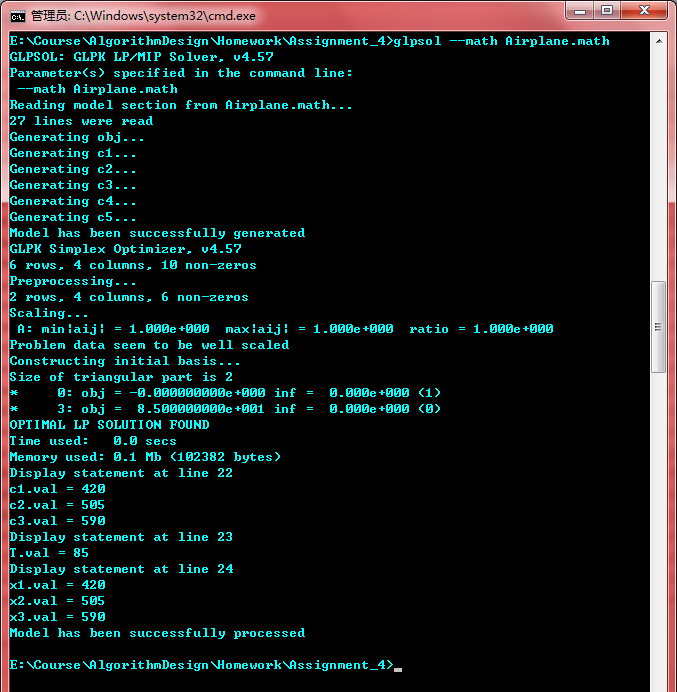
\includegraphics[width=0.75\columnwidth]{airplantresult} % Example image
        \end{center}
        More information reference the \emph{airplane.sol}
%
% Problem 2
%
\section{Gas Station Placement}
Let’s consider a long, quiet country road with towns scattered very sparsely
along it. Sinopec, largest oil refiner in China, wants to place gas stations along
the road. Each gas station is assigned to a nearby town, and the distance between any two gas stations being as small as possible. Suppose there are $n$
towns with distances from one endpoint of the road being $d_1,d_2, · · · ,d_n$. $n$ gas
stations are to be placed along the road, one station for one town. Besides, each
station is at most $r$ far away from its correspond town. $d_1,...,d_n$ and r have
been given and satisfied $d_1 < d_2 <...< d_n$, $0 < r < d_1$ and $d_i + r < d_{i+1} - r$
for all $i$. \\
The objective is to find the optimal placement such that the maximal distance between two successive gas stations is minimized.\\
Please formulate this problem as an LP.
\subsection{Formulate Problem}
From the question discription:
Assuption the $i$ gas statition at $s_i$, we should minimize the distance between two adjacent gas stations. \\
The Formalization as follows:
        \begin{equation}
             minimize: D
        \end{equation}
        s.t.
        \begin{equation}
        \begin{split}
             d_i - r \leq s_i \leq d_i + r    \\ where  i = 1.. n
        \end{split}
        \end{equation}
        \begin{equation}
        \begin{split}
             s_{i+1} - s_i \leq D       \\ where i = 1.. n-1
        \end{split}
        \end{equation}
        \begin{equation}
             s_{i+1} - s_i \leq T
        \end{equation}

The Slack form as follows:
        \begin{equation}
             minimize: D
        \end{equation}
        s.t.
        \begin{equation}
         s_i + a_1 =  r
        \end{equation}
        \begin{equation}
           - s_i + a_2 =  r - d_i
        \end{equation}
        \begin{equation}
         s_{i+1} - s_i - D + a_3 = 0 
        \end{equation}
        \begin{equation}
         a_1,a_2,a_3 \geq 0  
        \end{equation}
\subsection{Result}
        \begin{center}
            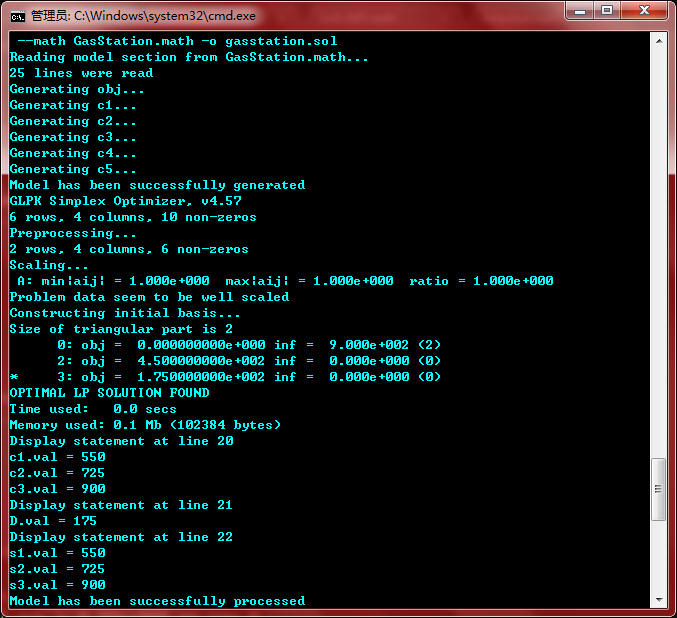
\includegraphics[width=0.75\columnwidth]{gasstationresult} % Example image
        \end{center}
        More information reference the \emph{gasstation.sol}

%
% Problem 3
%
\section{Simplex Algorithm}
Please implement simplex algorithm or dual simplex algorithm with your favorate language, and make comparison with GLPK or Gurobi or other similar tools.
\subsection{Simplex-Algorithm}
        \pythonscript{simplexity}{Simplex Algorithm using python implement}
\subsection{Comparion Result}
Test instance:\\
A = \\
                 [1, 1, 1, 1, 0, 0, 0]\\
                 [1, 0, 0, 0, 1, 0, 0]\\
                 [0, 0, 1, 0, 0, 1, 0]\\
                 [0, 3, 1, 0, 0, 0, 1]\\
b = 4,2,3,4 \\
c = 1,-14,-6, 0, 0, 0, 0 \\
\begin{center}
    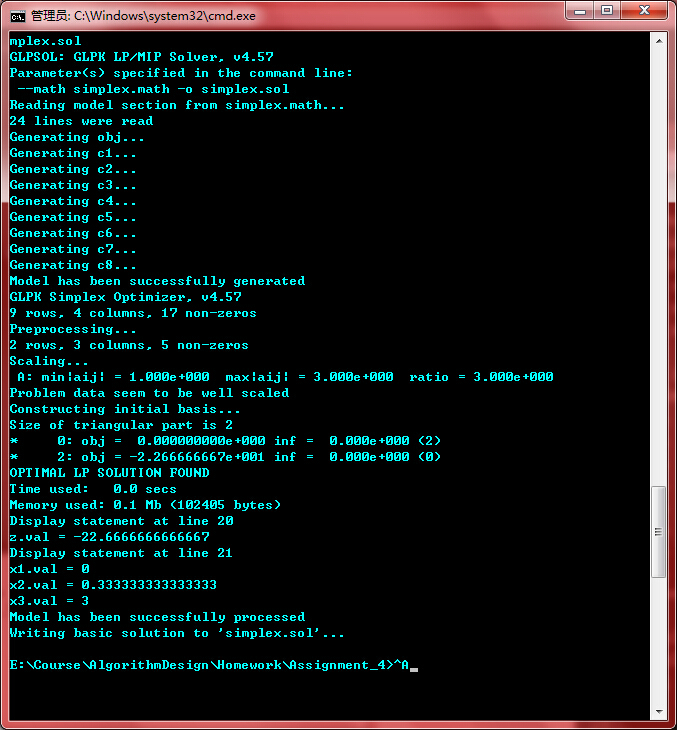
\includegraphics[width=0.75\columnwidth]{simplexresult} % Example image
\end{center}
Using my implement code, something error occur, there are something miss in pivot operation. It's odd that the basic of matrix A may become to less than expection number.

\end{document}
